\subsection{Another Question on a Kingdom}
\begin{frame}[t]{Another Question on a Kingdom}
\begin{columns}[T, onlytextwidth]
\column{0.5\textwidth}
\Moon\ 4 \Libra\ (L1) $\Rightarrow$ \Opposition\ \Saturn\ 11 \Aries\ in the 10th \textsl{"completes"} the matter as \Saturn\ receives the \Moon\ in his exaltation. \\
\vspace{0.5cm}
The man had little joy from his advancement; however, because \Saturn\ was in a place where he had no dignity, being in his Fall and furthermore, in a pitted degree and because it hated its own place it gave something hateful but it made what it gave fixed, strong, and stable because it was in an angle.
 
\column{0.5\textwidth}
\begin{center}
{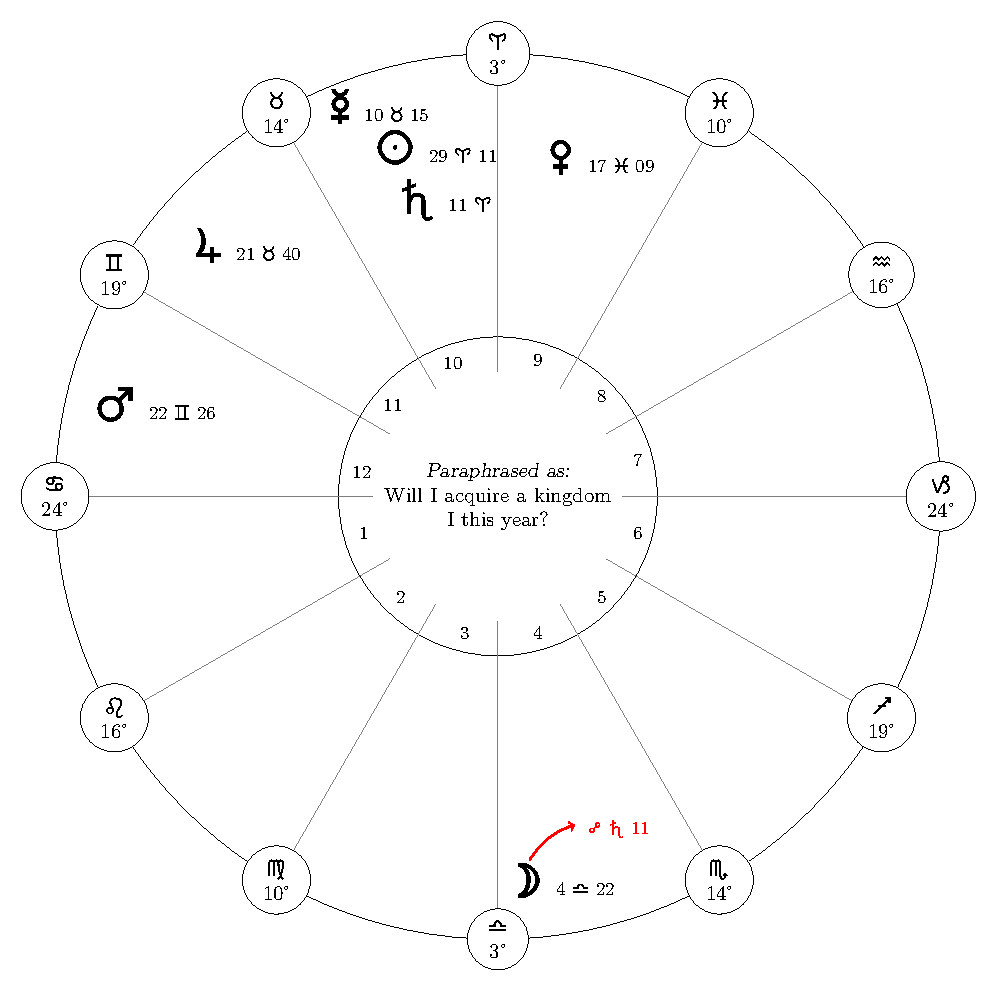
\includegraphics[width=0.9\textwidth]{charts/51-chart-kingdom}} \\
\end{center}
\end{columns}
\end{frame}